%%%%%%%%%%%%%%%%%%%%%%%%%%%%
% DOCUMENT SETUP & IMPORTS
%%%%%%%%%%%%%%%%%%%%%%%%%%%%
\documentclass[10pt,letterpaper,oneside,english]{article}
\usepackage[margin=.5in]{geometry}
\usepackage[utf8]{inputenc}
\usepackage{setspace}
	\onehalfspace


\usepackage{graphicx}

\usepackage{hyperref}

\usepackage{enumitem}
	\setenumerate[1]{label=\textit{\arabic*}}
	\setenumerate[2]{label=\textbf{\alph*},topsep=0pt}

%%%%%%%%%%%%%%%%%%%%%%%%%%%%
% USER-DEFINED COMMANDS
%%%%%%%%%%%%%%%%%%%%%%%%%%%%
% Usage: \person{<last>}{<first>}{<email>}
\newcommand{\person}[3]{
	#1, #2\\
	\href{mailto:#3}{\texttt{#3}}
}

% Usage: \teamMember{<name>}{<qualifications>}{<strengths>}
\newcommand{\teamMember}[3]{
	\textbf{#1}\\
	\textbf{Qualifications}: #2\\
	\textbf{Strengths}: #3
	\newline
	\newline
}

\newcommand{\see}[1]{(see {\color{blue!60!black}\nameref{#1}})}

\newcommand{\chref}[2]{\href{#1}{{\color{blue!60!black}#2}}}

\newcommand{\wref}{\href{http://en.wikipedia.org/wiki/Main_Page}{({\color{blue!60!black}from Wikipedia})}}

\newcommand{\solution}{\newline \hspace*{1em} \textbf{Solution: }}

\newcommand{\code}[1]{\texttt{#1}}

\newcommand{\citem}[1]{\item \code{#1}}

\newcommand{\gls}[2]{ \ \\ \hspace*{1em} \textbf{#1} \ \\ \hspace*{1.5em}{#2}}


%%%%%%%%%%%%%%%%%%%%%%%%%%%%
% TITLE AUTHORS AND DATE
%%%%%%%%%%%%%%%%%%%%%%%%%%%%
\title{
	\textbf{Game Engine Development Team}\\
	Design Specification v1.0
}

\author{
	\person{Bahr}{Dan}{dbahr92@gmail.com}
	\and
	\person{Bard}{Etan}{ebard@ups.edu}
	\and
	\person{Burns}{Nick}{nbburns@ups.edu}
	\and
	\person{Livingston}{Chris}{christopherlivingston92@gmail.com}
	\and
	\person{Wilson}{Robin}{rkwilson@ups.edu}
}
\date{\today}



%%%%%%%%%%%%%%%%%%%%%%%%%%%%
% DOCUMENT
%%%%%%%%%%%%%%%%%%%%%%%%%%%%
\begin{document}
\maketitle
\newpage

\tableofcontents
\newpage

\section{Introduction}
This document details the internal architecture of the game, as detailed in the  Requirements Specification document.

The game design team will create an interesting and entertaining game that can be played as a stand-alone system, as well as fit into the larger Vi-Char system. Our group is responsible for generating the game world where the character exists. The character will be able to: pick up items, navigate the world by jumping and moving, and fight floating creatures (controlled by the mobile device users iif available). These floating creatures can directly harm the Character by shooting fireballs towards the character and indirectly by spawning enemies, moving an attacking turret, and delete the ground that the Character walks on. Scores of the character and floating creatures will be tracked.
The game will receive inputs from the Motion Capture group directly, and Mobile Device group via the Web Server. These inputs will be translated into actions made by the Character and floating creatures respectively. Scores will be sent to the Web Server.

\section{Architecture Design} 
The game engine, running in Unity3D will be located on a desktop, separate from other parts of Vi-Char. A Kinect, a keyboard, and projector will be connected to this machine. The computer will also have an internet connection for communication purposes.

Three major modules will exist inside the machine i.e. the GameWorld, InputControls, and Network. The GameWorld includes several classes: the CharacterClass, CameraClass, EnemyClass, ItemsInterface, FloatingCreature, and PlatformsClass. GameWorld from a high-level standpoint monitors the state of all game objects, such as the state of the platforms and items. InputControls is the interface for the Kinect group, which takes magnitudes and actions from the Kinect group and transforms these into character actions. The network interfaces with the Web Server, providing updates for the Mobile Devices in the GameWorld such character data and scores. What the Network recieves from the Server are mobile device positions and actions for the floating creatures to do.

The GameWorld module encompasses a vast array of classes. The CharacterClass is responsible for using the information from the InputControls module and determining the actions of the character. The CameraClass will provide the MainDisplay with a view of the game world for spectators and the puppeteers. EnemyClass provides the artificial intelligence for floating opponents that are not controlled by Mobile Users as well as attacking turrets and spawned enemies. ItemsInterface provides a blueprint for which the Character’s state can be modified by picking up consumables that are collected in the game-environment. The FloatingCreature class is responsible for tracking the Mobile Devices’ positions and rendering the floating creature characters for Camera to see. Finally, the PlatformsClass is responsible for monitoring the state of all tiles in the game world, and for modifications of the tiles by events that occur in the game.


\section{Module Design}
\subsection{Overview of V-Char}
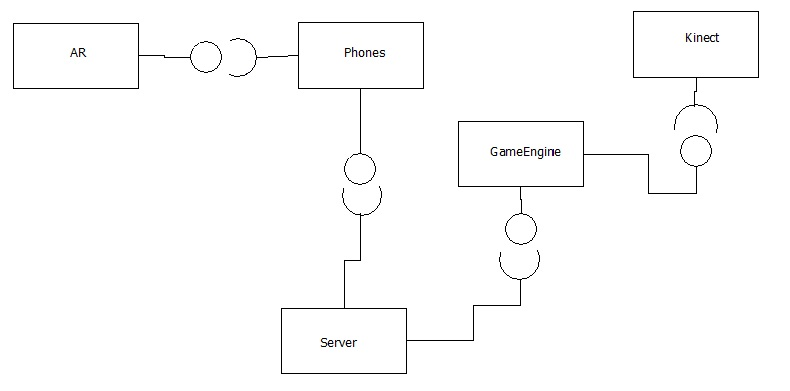
\includegraphics[scale=0.7]{overview}
\subsection{Diagram of the game engine}
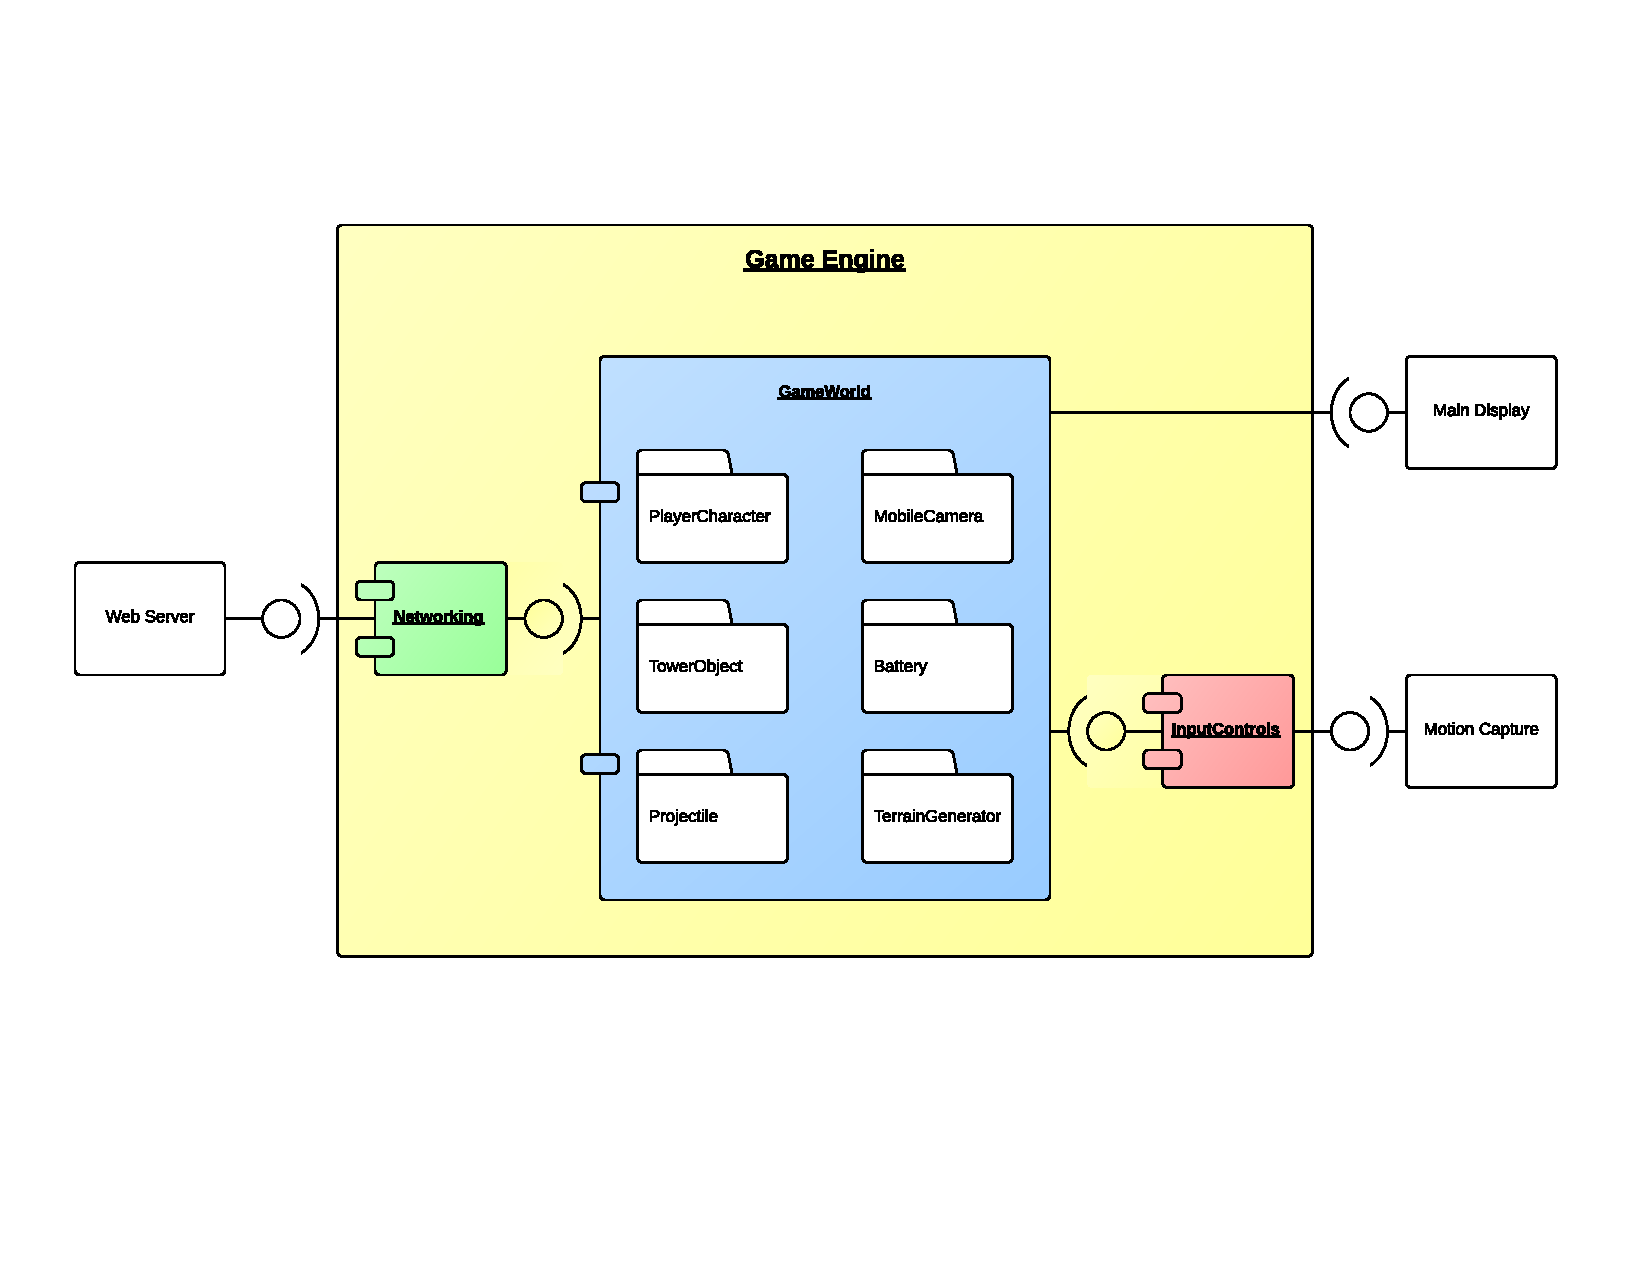
\includegraphics[scale=0.7]{ComponentDiagram}
\subsection{InputControls}
\subsubsection{Description}
	The InputControls module contains individual functions for specific tasks (see Provided Interface). These functions will be called in order to move the Character or have the Character perform an action. Thus, the InputControls module is the interface between the character movements and the outside world.
\subsubsection{Purpose}
	This module is responsible for consolidating all of the actions that a Character can perform. It will allow us to control the Character from multiple inputs simultaneously and will be used primarily as an interface between the game engine and the motion capture.
\subsubsection{Provided Interface}
Functions for controlling the Character. Examples:
\begin{enumerate}
		\citem {void Jump(float magnitude);}
		\citem {void MoveForward(float magnitude);}
		\citem {void MoveBackward(float magnitude);}
		\citem {void MoveLeft(float magnitude);}
		\citem {void MoveRight(float magnitude);}
		\citem {void PrimaryAttack();}
		\citem {void SecondaryAttack();}
		\citem {void Shield();}

	\end{enumerate}
\subsubsection{Required Interface}
\texttt{getKinectActions();}

\subsection{GameWorld}

\subsubsection{Description}
The game world is our main module. This module includes several classes: CharacterClass, CameraClass, Enemy, Items, PowerUps, and Platforms. These classes will interact with each other to simulate the game world. For example, an Enemy might attack an instance of the CharacterClass, and the character may pick up an item and use it to destroy the enemy. All of this interaction occurs in the GameWorld module.

\subsubsection{Purpose}
	The GameWorld module essentially keeps track of the static and dynamic objects and where exactly the Character is in the world. The GameWorld is responsible for getting inputs from the InputControl Module for the Character and getting inputs from the Network Module for where the FloatingCreatures are. This module will also take care of rendering the game world and the background. Sound will also be a sub-module of the GameWorld. The GameWorld will spawn batteries and items depending on what the Web Server group gets on twitter. 

\subsubsection{Provided Interface}
\begin{enumerate}
	\citem Character direction and position, object placement, enemy direction and placement. 
	\citem Game-world display for MainDisplay
\end{enumerate}
\subsubsection{Required Interface}
\begin{enumerate}
	\item Object creation and placement from Network Module (Web Server group)
	\item Twitter inputs from Network Module(Web Server Group)
	\item \code{getActions()} from InputController Module
	\item \code{getMobileDevicePosition()} from Network Module (Server group)
\end{enumerate}

\subsection{Classes Inside GameWorld Module}

\subsection{CharacterClass}

\subsubsection{Description}
	The CharacterClass module will keep track of the character in game and will take the inputs from the MotionCapture group and will call animations accordingly. Since there is only one Character in the GameWorld, there will be no subclasses of Character. 

\subsubsection{Purpose}
	The CharacterClass module provides the code-based structure of the in-game Character. It is the representation of the Character within the code. Everything that happens to the Character will be a byproduct of what is designed in this class.

\subsubsection{Examples of Functions}
\begin{enumerate}
		\item Functions for controlling the finer granularities of the Character or for retrieving specific information about the Character.
		\citem {void DoAnimation(AnimationType aType);}
		\citem {Vector3 GetLocation();}
	\end{enumerate}

\subsubsection{Required Interface}
	\code{getActions()} from Motion Capture

\subsection{CameraClass}

\subsubsection{Description}
The camera will provide a view of the game world to be displayed on the MainDisplay. Since there is only one camera in the game environment that will be exclusively following the Character, the Camera will not have any subclasses.

\subsubsection{Purpose}
	The Camera module encapsulates the movement of the camera in the game world. This camera is the one through which the game is viewed by the puppeteers (i.e. is it the viewport for the game as viewed on a computer monitor or projector). This module allows us to control the camera from multiple other modules at the same time. For example, the camera may always follow within a certain distance of the Character’s location, but the user may want to rotate the camera via the InputControls module. 

\subsubsection{Examples of Functions}
Functions for rotating the camera around the Character and moving the camera in world-space. This calculation will be made inside this class.
\begin{enumerate}
		\citem {void Rotate(float distanceDegrees);}
		\citem {void Move(Vector3 location);}
		\citem {void DisplayWorld();}
\end{enumerate}

\subsubsection{Required Interface}
	A mechanism for getting the location of the Character (as provided by the Character Class).

\subsection{Other Classes inside GameWorld}

\subsubsection{ItemsInterface}
Every item in the GameWorld will implement this interface. Item classes will spawn all over the game world that the Character will be able to pick up and utilize, or change the state of the Character. For example, the Character may be able to move faster after collecting a certain item.

\subsubsection{EnemyClass}
The EnemyClass will contain an AI to fight the Character that the Floating Creatures can spawn at will to fight the Character. 

\subsubsection{Floating Creature}
This class will update where the Mobile Devices are in the GameWorld (getting the positions of the phones from the Server) so that when the CameraClass displays where the Mobile Users’ phones are, the MainDisplay will show a Floating Creature at the corresponding location in the game world.

\subsubsection{PlatformClass}
The PlatformClass will describe the different types of platforms the GameWorld can have. They can be deleted or modified.

\subsection{Network}

\subsubsection{Purpose}
	The Network module encapsulates everything concerning networked communications and speaking to the web server. It will provide functions for sending data in a clear manner with a well-defined API that can be used from within the other functions. It will automatically send the Character position provided by the CharacterController module and will send object data from the GameWorld module. It will provide an interface for receiving data from the server as well (such as data about new augmented reality objects).

\subsubsection{Provided Interface}
Functions for getting data from the server:
\begin{enumerate}
\citem {ARData GetNewARData();}
\end{enumerate}

\subsubsection{Required Interface}
	Functions for retrieving the character position (provided by the CharacterController module) and for retrieving object data (provided by the GameWorld module).

\section{Other Design Views} 


\subsection{Integration with Motion Capture}

The Motion Capture group has the most direct interaction with the Game Design group. We have assumed that the Motion Capture group will write their code within Unity, thus making integration relatively simple. In our design, the motion capture group will send motion data to the game engine by calling functions that we offer. Examples of such functions include void Move(float distanceForward) or void RotateLeft(float rotation). These functions (managed by the InputControls module) will later be used by the game engine to control the movement of the character. From the Motion Capture group’s point of view, however, all they will need to do is call the appropriate function in the InputControls module to move the character accordingly.

\subsection{Integration with Web Server/Mobile Devices}

From our point of view, the Web Server is merely the transport for communication between the Game Design group and the Mobile Device group. We will be communicating via HTTP with the server and assume that such communications are forwarded on to the mobile devices as appropriate. An example of communication that will be sent to the phones will be character data (such as position and the direction the character is facing). We will also receive data from the phones via the server such as augmented reality data (for buildings, obstacles, and the like). All network communication will be done via the NetworkingInterface module which communicates with the web server directly. With the assumption that the web server uses HTTP, this module will abstract the process of building and sending HTTP “GET” and “POST” requests. Because the Game Design group will be polling for data in this manner, the Web Server need not know about us at all. The web server supplies the interface for networked communication, and the game engine uses this interface via the NetworkingInterface module.

\section{Design Rationale}

\subsection{Rationale behind the GameWorld module}

The GameWorld control module is the module we will be relying on most. All of the other modules will modify everything that is done in this module. The reason this module will be made up of several classes because it is easier to store information and do system calls to each class inside one entity. For all intensive purposes, the GameWorld module takes everything we need from the other groups and utilizes the inputs to play the game. 

\subsection{Rationale behind the InputControls module}

To reiterate, the InputControls module provides the mechanism for taking any sort of input from the user and moving the character accordingly. The reasoning for this is to make it simple to use any user input, whether a keyboard, motion capture, or a gamepad. Thus, the input from the user will act as ``plug and play'', where the user can choose to play how he/she/they prefer. This also means that the game could be played without motion capture, via the keyboard. The InputControls module fulfills the requirements specification for player interaction in the game world via motion capture.

\subsection{Rationale behind the CameraClass}

The CameraClass provides the means for moving the main camera for the MainDisplay, thus altering the viewport through which the game is viewed. This is a class inside GameWorld so that the main viewport for the game can be changed from multiple other parts inside the if necessary (for example, perhaps the camera is always behind the character and is controlled by the CharacterClass, or perhaps the user can rotate the camera by using a motion or a joystick).

\subsection{Rationale behind the Networking Module}

The Network Module will be a black box for everything related to networked communications. It will provide well-named functions and a simple API that the other modules may use for sending and receiving data. The black box abstracts away all of the “guts” of networked communications. This module will be used to fulfill the requirement specifications involved with the web server and mobile devices.

\section{Implementation Notes}
The game will be implemented using a variety of tools. 
Unity3D will be used to control the 3D game content, including game-state management, and intercommunication with the motion and mobile groups. Complex game models such as the character and the floating creatures will be created using Blender and open source animation and 3D modeling program. Using the Blender FBX exporter we can take the models created in Blender and insert them into Unity. Game models will be directed by Unity3D, according to appropriate inputs. Unity3D provides Kinect integration and network interfaces, allowing input collection.
Github will be used to host source code in a central repository. Data will be transferred with the git distributed version control system.
Documentation will be prepared with a hosted collaborative text editor such as Google Docs. Documentation may or may not be prepared with the use of LaTeX, a document markup language and preparation system.

\section{Glossary and References}

\gls{Avatar}{See Character}

\gls{Character}{The game object controlled by persons using the Kinect}

\gls{Floating Creatures}{The avatars inside the GameWorld the Mobile Device group control}

\gls{Gamepad}{A human input device with buttons and analog sticks}

\gls{git}{A distributed version control system, which tracks and annotates changes to }code

\gls{Github}{A hosting service for the source code of software projects}

\gls{Google Docs}{A service provided by Google to collaboratively create documents}

\gls{Kinect}{A motion capture system, gathers 3D information of puppeteer's locations}

\gls{LaTeX}{A document markup language and preparation system}

\gls{MainDisplay}{The projector that spectators as well as puppeteers will be able to see. Will display the current state of the gameworld.}

\gls{Unity3D}{Integrated authoring tool for creating 3D video games or other interactive content such as architectural visualizations or real-time 3D animations}

\gls{Viewport}{The view seen of the game, similar to an aerial view}


\end{document}
